\documentclass{article}
\usepackage{amsmath}
\usepackage{tikz}
\usepackage[margin=1in]{geometry}

\begin{document}

\title{Ruta más corta}
\author{}
\date{\today}

\maketitle
\section*{Problema}

Los nodos de la siguiente red representan distintas ciudades de un país que nadie conoce y los arcos son todos los caminos (dirigidos) posibles por recorrer. Los valores sobre los arcos representan las distancias en kilómetros entre ciudades. Un camión repartidor debe entregar producto desde la fábrica que está en la ciudad \( X \) hasta la tienda minorista que está ubicada en la ciudad \( Z \). Determine la ruta más corta para poder efectuar la entrega.

\begin{center}
    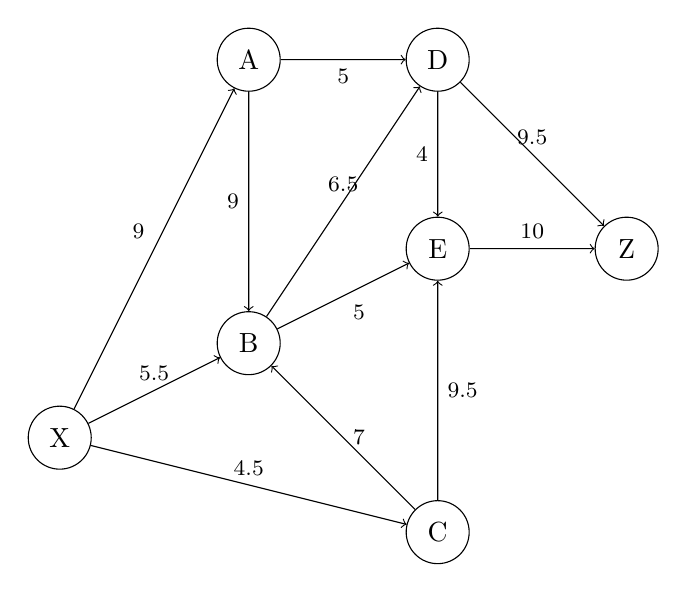
\begin{tikzpicture}[scale=1.2, node/.style={circle, draw, minimum size=0.8cm}]
        % Nodos
        \node[node] (X) at (0, 0) {X};
        \node[node] (A) at (2, 4) {A};
        \node[node] (B) at (2, 1) {B};
        \node[node] (C) at (4, -1) {C};
        \node[node] (D) at (4, 4) {D};
        \node[node] (E) at (4, 2) {E};
        \node[node] (Z) at (6, 2) {Z};

        % Arcos y pesos
        \draw[->] (X) -- (A) node[midway, above left] {\footnotesize 9};
        \draw[->] (X) -- (B) node[midway, above] {\footnotesize 5.5};
        \draw[->] (X) -- (C) node[midway, above] {\footnotesize 4.5};
        \draw[->] (A) -- (B) node[midway, left] {\footnotesize 9};
        \draw[->] (A) -- (D) node[midway, below] {\footnotesize 5};
        \draw[->] (B) -- (D) node[midway, above] {\footnotesize 6.5};
        \draw[->] (B) -- (E) node[midway, below right] {\footnotesize 5};
        \draw[->] (C) -- (B) node[midway, right] {\footnotesize 7};
        \draw[->] (C) -- (E) node[midway, right] {\footnotesize 9.5};
        \draw[->] (D) -- (E) node[midway, left] {\footnotesize 4};
        \draw[->] (D) -- (Z) node[midway, above] {\footnotesize 9.5};
        \draw[->] (E) -- (Z) node[midway, above] {\footnotesize 10};
    \end{tikzpicture}
\end{center}

\textbf{Solución.}
Para determinar la ruta más corta desde la ciudad \( X \) hasta la ciudad \( Z \) en el grafo proporcionado, utilizaremos el algoritmo de Dijkstra, que es un método eficiente para encontrar el camino de menor costo en un grafo con arcos de peso no negativo.

\section*{Paso 1: Inicialización}

\begin{itemize}
    \item Establecemos la distancia inicial desde \( X \) a sí mismo como 0.
    \item Todas las demás distancias iniciales a infinito.
    \item Creamos un conjunto de nodos no visitados que incluye todas las ciudades.
\end{itemize}

\section*{Paso 2: Iteración del Algoritmo}

\begin{itemize}
    \item \textbf{Nodo Actual: \( X \)}
    \begin{itemize}
        \item \textbf{Vecinos de \( X \):}
        \begin{itemize}
            \item \( X \rightarrow A \): distancia acumulada = \( 0 + 9 = 9 \)
            \item \( X \rightarrow B \): distancia acumulada = \( 0 + 5.5 = 5.5 \)
            \item \( X \rightarrow C \): distancia acumulada = \( 0 + 4.5 = 4.5 \)
        \end{itemize}
        \item Actualizamos las distancias mínimas:
        \begin{itemize}
            \item \( \text{dist}(A) = 9 \)
            \item \( \text{dist}(B) = 5.5 \)
            \item \( \text{dist}(C) = 4.5 \)
        \end{itemize}
        \item Marcamos \( X \) como visitado.
    \end{itemize}

    \item \textbf{Nodo Actual: \( C \) (distancia mínima actual: 4.5)}
    \begin{itemize}
        \item \textbf{Vecinos de \( C \):}
        \begin{itemize}
            \item \( C \rightarrow B \): distancia acumulada = \( 4.5 + 7 = 11.5 \) (no mejora la distancia existente a \( B \))
            \item \( C \rightarrow E \): distancia acumulada = \( 4.5 + 9.5 = 14 \)
        \end{itemize}
        \item Actualizamos la distancia mínima:
        \begin{itemize}
            \item \( \text{dist}(E) = 14 \)
        \end{itemize}
        \item Marcamos \( C \) como visitado.
    \end{itemize}

    \item \textbf{Nodo Actual: \( B \) (distancia mínima actual: 5.5)}
    \begin{itemize}
        \item \textbf{Vecinos de \( B \):}
        \begin{itemize}
            \item \( B \rightarrow D \): distancia acumulada = \( 5.5 + 6.5 = 12 \)
            \item \( B \rightarrow E \): distancia acumulada = \( 5.5 + 5 = 10.5 \)
        \end{itemize}
        \item Actualizamos las distancias mínimas:
        \begin{itemize}
            \item \( \text{dist}(D) = 12 \)
            \item \( \text{dist}(E) = 10.5 \) (mejora sobre la distancia anterior)
        \end{itemize}
        \item Marcamos \( B \) como visitado.
    \end{itemize}

    \item \textbf{Nodo Actual: \( A \) (distancia mínima actual: 9)}
    \begin{itemize}
        \item \textbf{Vecinos de \( A \):}
        \begin{itemize}
            \item \( A \rightarrow D \): distancia acumulada = \( 9 + 5 = 14 \) (no mejora la distancia existente a \( D \))
        \end{itemize}
        \item Marcamos \( A \) como visitado.
    \end{itemize}

    \item \textbf{Nodo Actual: \( E \) (distancia mínima actual: 10.5)}
    \begin{itemize}
        \item \textbf{Vecinos de \( E \):}
        \begin{itemize}
            \item \( E \rightarrow Z \): distancia acumulada = \( 10.5 + 10 = 20.5 \)
        \end{itemize}
        \item Actualizamos la distancia mínima:
        \begin{itemize}
            \item \( \text{dist}(Z) = 20.5 \)
        \end{itemize}
        \item Marcamos \( E \) como visitado.
    \end{itemize}

    \item \textbf{Nodo Actual: \( D \) (distancia mínima actual: 12)}
    \begin{itemize}
        \item \textbf{Vecinos de \( D \):}
        \begin{itemize}
            \item \( D \rightarrow Z \): distancia acumulada = \( 12 + 9.5 = 21.5 \) (no mejora la distancia existente a \( Z \))
        \end{itemize}
        \item Marcamos \( D \) como visitado.
    \end{itemize}

    \item \textbf{Nodo Actual: \( Z \) (distancia mínima actual: 20.5)}
    \begin{itemize}
        \item Marcamos \( Z \) como visitado.
    \end{itemize}
\end{itemize}

\section*{Paso 3: Reconstrucción de la Ruta Más Corta}

\begin{itemize}
    \item Desde \( Z \), retrocedemos utilizando los nodos previos guardados durante la actualización de distancias:
    \begin{itemize}
        \item \( Z \) viene de \( E \)
        \item \( E \) viene de \( B \)
        \item \( B \) viene de \( X \)
    \end{itemize}
\end{itemize}

La ruta más corta es: \( X \rightarrow B \rightarrow E \rightarrow Z \)

\section*{Conclusión}

La ruta más corta desde \( X \) hasta \( Z \) es pasando por \( B \) y \( E \), con una distancia total de \textbf{20.5 kilómetros}.

\textbf{Ruta más corta:} \( X \rightarrow B \rightarrow E \rightarrow Z \), con una distancia total de 20.5 kilómetros.

\end{document}
